\documentclass[10pt]{beamer}
\usetheme[block=fill]{metropolis} % Use metropolis theme with colored blocks
\usepackage[spanish]{babel}
\usepackage[utf8]{inputenc}
\usepackage{graphicx}
\usepackage{booktabs}
\usepackage{caption}

\title{Estudio de Técnicas de Aprendizaje Automático usando Sobremuestreo de Datos}
\date{\today}
\author{Aarón Zeballo \\ Tutora: Dra. Andrea Rey}
\institute{Universidad Nacional de Hurlingham}

\titlegraphic{\hfill
\includegraphics[height=1.5cm]{logo.jpg}}

\begin{document}

\maketitle

\section{Planteamiento del Problema}

\begin{frame} {Correo No Deseado (Spam)}
  \begin{itemize}
    \item \textbf{Evolución Histórica:} Lo que comenzó como publicidad molesta en los 90 evolucionó a una de las principales herramientas del cibercrimen moderno.
    \item \textbf{Impacto Actual:} 
    \begin{itemize}
        \item Saturación de infraestructura y daño económico a nivel corporativo.
        \item Riesgo de seguridad y estafas para usuarios.
    \end{itemize}
    \item \textbf{El rol del Machine Learning:} Los filtros basados en reglas estáticas quedaron obsoletos. Se requieren algoritmos capaces de detectar patrones.
    \item El Gran Desafío: Entrenar estos modelos presenta un problema debido a los correos: el desbalanceo entre los legítimos y los de \textit{spam}.
  \end{itemize}
\end{frame}

\begin{frame}{Desbalanceo de Clases}
  \begin{itemize}
    \item Los correos legítimos son la mayoría; las amenazas, la minoría.
    \item Para simular un entorno real, se eliminaron instancias de la clase \textit{spam} hasta alcanzar un porcentaje del 5\%.
  \end{itemize}
  \begin{figure}
    \centering
    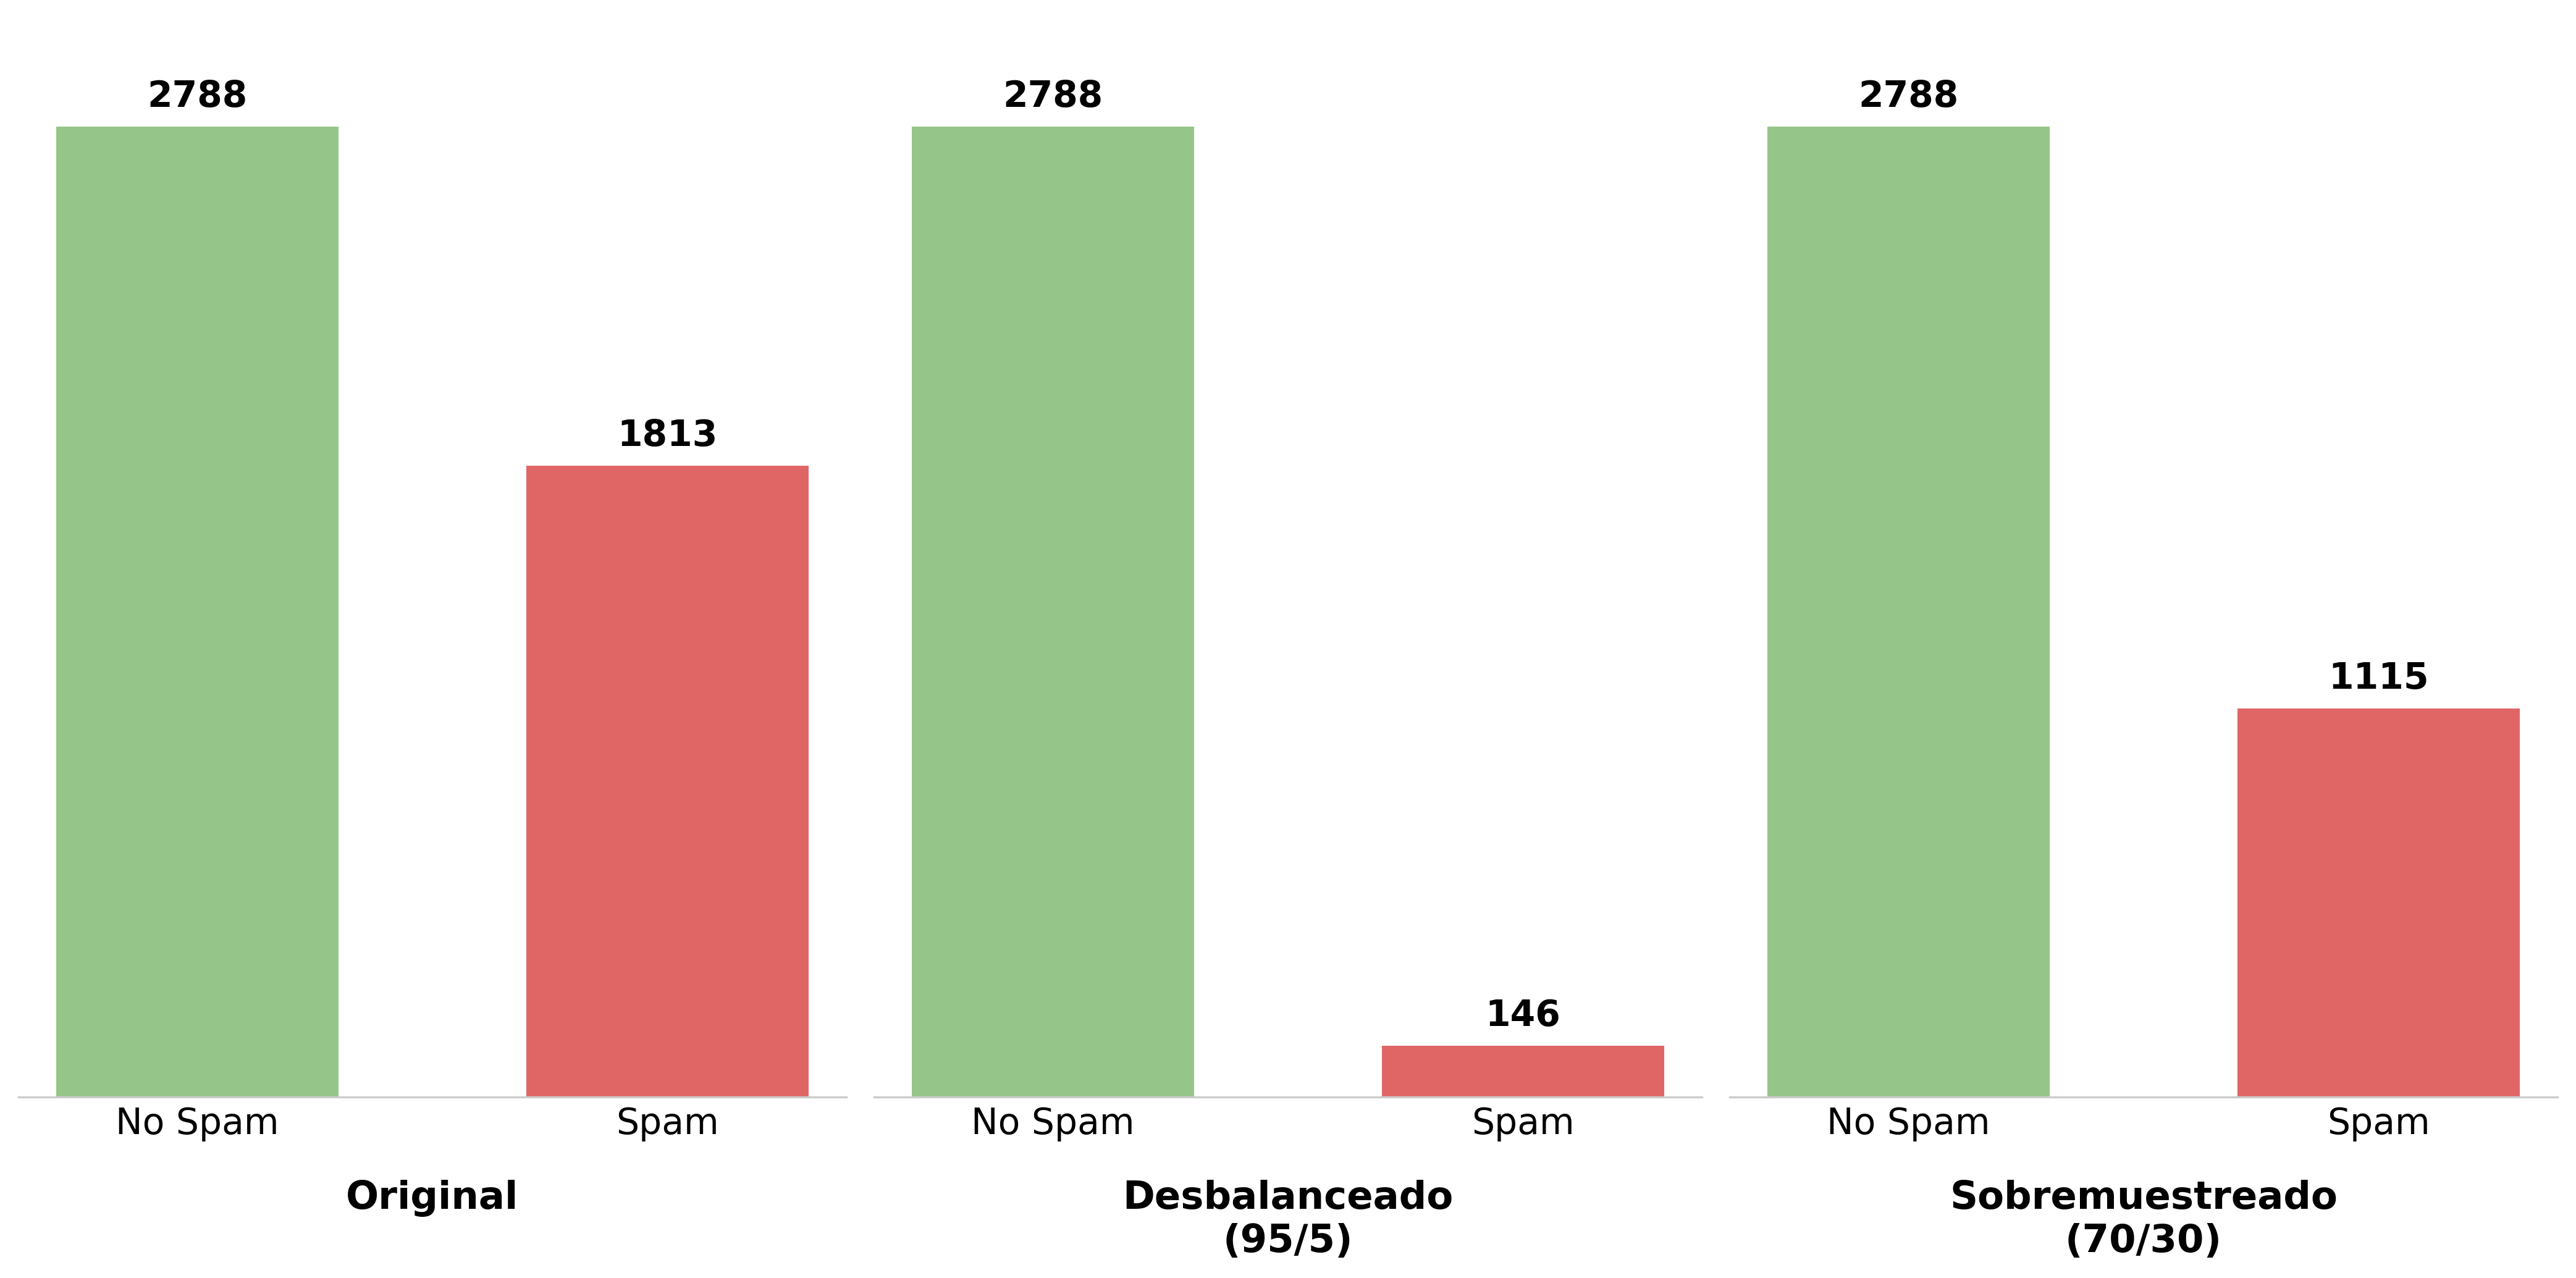
\includegraphics[width=0.9\textwidth]{distribucion_clases_barras.png}
  \end{figure}
\end{frame}


\begin{frame}{Conjunto de Datos (Spambase)}
  Dataset público estructurado con 57 características predictoras continuas extraídas mediante procesamiento de texto:
  \vspace{0.3cm}
  \begin{table}
    \centering
    \small
    \begin{tabular}{@{}llp{5cm}@{}}
      \toprule
      \textbf{Familia de Variables} & \textbf{Atributos} & \textbf{Ejemplo / Unidad} \\
      \midrule
      Frecuencia de palabras & 48 & \texttt{word\_freq\_free} (\%) \\
      Frecuencia de caracteres & 6 & \texttt{char\_freq\_\$} (\%) \\
      Secuencia de mayúsculas & 3 & \texttt{capital\_run\_length\_total} (Conteo Absoluto) \\
      \midrule
      \textbf{Variable Objetivo} & \textbf{1} & Legítimo (0) o Spam (1) \\
      \bottomrule
    \end{tabular}
  \end{table}
\end{frame}
\section{Métodos Utilizados}



\begin{frame}{Uso de StandardScaler}
  \begin{itemize}
    \item \textbf{Problema de Escalas:} Las variables de frecuencia de palabras están en porcentajes (0 a 5\%), mientras que la secuencia de mayúsculas es un conteo absoluto (llegando a miles).
    \item \textbf{Consecuencia:} SVM sufre en su calidad predictiva dando atención casi exclusiva a las mayúsculas.
    \begin{itemize}
        \item Transforma las variables para tener Media = 0 y Varianza = 1.
        \item Ajustado exclusivamente sobre datos de entrenamiento para evitar Data Leakage.
        \item Restaura la capacidad del algoritmo para evaluar todas las variables.
    \end{itemize}
  \end{itemize}
\end{frame}

\section{Técnicas de sobremuestreo}

\begin{frame}{Técnica de sobremuestreo: SMOTE}
  \textbf{Synthetic Minority Over-sampling Technique}
  \begin{itemize}
    \item Algoritmo estándar en la industria para la creación de datos sintéticos.
    \item Analiza instancias de la clase minoritaria (spam) y busca a sus $k$ vecinos más cercanos ($k=5$).
    \item Genera nuevos ejemplos trazando líneas rectas entre el ejemplo original y los vecinos elegidos al azar que sean necesarios.
    \item Desventaja: Genera datos uniformemente para toda la clase minoritaria, lo que puede perjudicar al clasificador si la línea cruza por zonas de correos legítimos.
  \end{itemize}
\end{frame}

\begin{frame}{Técnica de sobremuestreo: G-SMOTE}
  \textbf{Geometric SMOTE}
  \begin{itemize}
    \item Evolución geométrica para evitar la creación de instancias en zonas de la clase contraria.
    \item En lugar de generar muestras sobre líneas rectas, define una zona esférica alrededor de los correos minoritarios originales.
    \item Su precisión radica en calcular primero la distancia exacta hacia el ejemplo legítimo más cercano, restringiendo el radio de la esfera para nunca cruzar esa frontera.
    \item Resulta en un sobremuestreo seguro, sin invadir el territorio  de correos legítimos.
  \end{itemize}
\end{frame}

\begin{frame}{Técnica de sobremuestreo: ADASYN}
  \textbf{Adaptive Synthetic Sampling}
  \begin{itemize}
    \item Evolución que corrige el problema de SMOTE prestando mucha atención a las fronteras de decisión.
    \item Calcula la densidad de probabilidad para definir qué tan ``difícil" de aprender es cada instancia de spam.
    \item Concentra la creación de datos artificiales únicamente alrededor de los correos más difíciles de clasificar.
    \item Ventaja: Evita generar información en zonas que los modelos ya pueden separar fácilmente.
  \end{itemize}
\end{frame}



\begin{frame}{Técnica de sobremuestreo: ADASYN + ENN}
  \textbf{Método Híbrido (Edited Nearest Neighbours)}
  \begin{itemize}
    \item Combina ADASYN con una  etapa de limpieza  final (ENN).
    \item \textbf{Fase 1:} ADASYN inyecta nuevos datos sintéticos en las zonas más difíciles de clasificar.
    \item \textbf{Fase 2:} El algoritmo ENN revisa todo el conjunto ampliado evaluando a los 3 vecinos más cercanos de cada observación.
    \item Si detecta que una instancia está rodeada por la clase contraria, asume que confundirá al clasificador y la elimina por completo.
  \end{itemize}
\end{frame}

\section{Modelos de Clasificación}

\begin{frame}{Modelos de Clasificación: Parámetros}
  \begin{columns}[T]
    
    % Columna 1: Árbol de Decisión
    \begin{column}{0.33\textwidth}
      \begin{block}{Árbol de Decisión}
        \vspace{0.1cm}
        \scriptsize
        \textbf{Criterio de partición:}\\ \texttt{gini} \\[1.5ex]
        \textbf{Profundidad máxima:}\\ \texttt{Ninguna} \\[1.5ex]
        \textbf{Muestras mín. dividir:}\\ 2 \\[1.5ex]
        \textbf{Muestras mín. hoja:}\\ 1
        \vspace{0.1cm}
      \end{block}
    \end{column}

    % Columna 2: Random Forest
    \begin{column}{0.33\textwidth}
      \begin{exampleblock}{Random Forest}
        \vspace{0.1cm}
        \scriptsize
        \textbf{Criterio de partición:}\\ \texttt{gini} \\[1.5ex]
        \textbf{Cantidad de árboles:}\\ 100 \\[1.5ex]
        \textbf{Caract. división:}\\ \texttt{Raíz cdra.} \\[1.5ex]
        \textbf{Muestras mín. dividir:}\\ 2
        \vspace{0.1cm}
      \end{exampleblock}
    \end{column}

    % Columna 3: SVM
    \begin{column}{0.33\textwidth}
      \begin{alertblock}{SVM}
        \vspace{0.1cm}
        \scriptsize
        \textbf{Regularización (C):}\\ 1.0 \\[1.5ex]
        \textbf{Tipo de Kernel:}\\ \texttt{rbf} \\[1.5ex]
        \textbf{Coeficiente Kernel:}\\ \texttt{scale} \\[1.5ex]
        \textbf{Umbral Decisión:}\\ 0.2
        \vspace{0.1cm}
      \end{alertblock}
    \end{column}

  \end{columns}
  
  \vspace{0.3cm}
  \begin{center}
      \scriptsize \textit{* Se utilizaron los parámetros por defecto de \texttt{scikit-learn}, únicamente cambiando manualmente el umbral de decisión del SVM a \textbf{0,2}}
  \end{center}
\end{frame}

\section{Resultados}





\begin{frame}{Justificación de la Proporción Óptima}
  Se evaluaron múltiples niveles de sobremuestreo para encontrar el equilibrio ideal:
  \vspace{0.3cm}
  \begin{table}
    \centering
    \small
    \begin{tabular}{@{}lccc@{}}
      \toprule
      \textbf{Proporción (Legítimo/Spam)} & \textbf{Precision} & \textbf{Recall} & \textbf{F1-Score} \\
      \midrule
      50-50 & 0,5556 & 0,8621 & 0,6757 \\
      60-40 & 0,6098 & 0,8621 & 0,7143 \\
      \textbf{70-30} & \textbf{0,6757} & \textbf{0,8621} & \textbf{0,7576} \\
      80-20 & 0,6471 & 0,7586 & 0,6984 \\
      \bottomrule
    \end{tabular}
  \end{table}
  
  \vspace{0.2cm}
  La relación 70-30 aumenta el F1-Score sin sacrificar Recall.
\end{frame}

\begin{frame}{Resultados con Proporción Óptima (70-30)}
  \begin{figure}
    \centering
    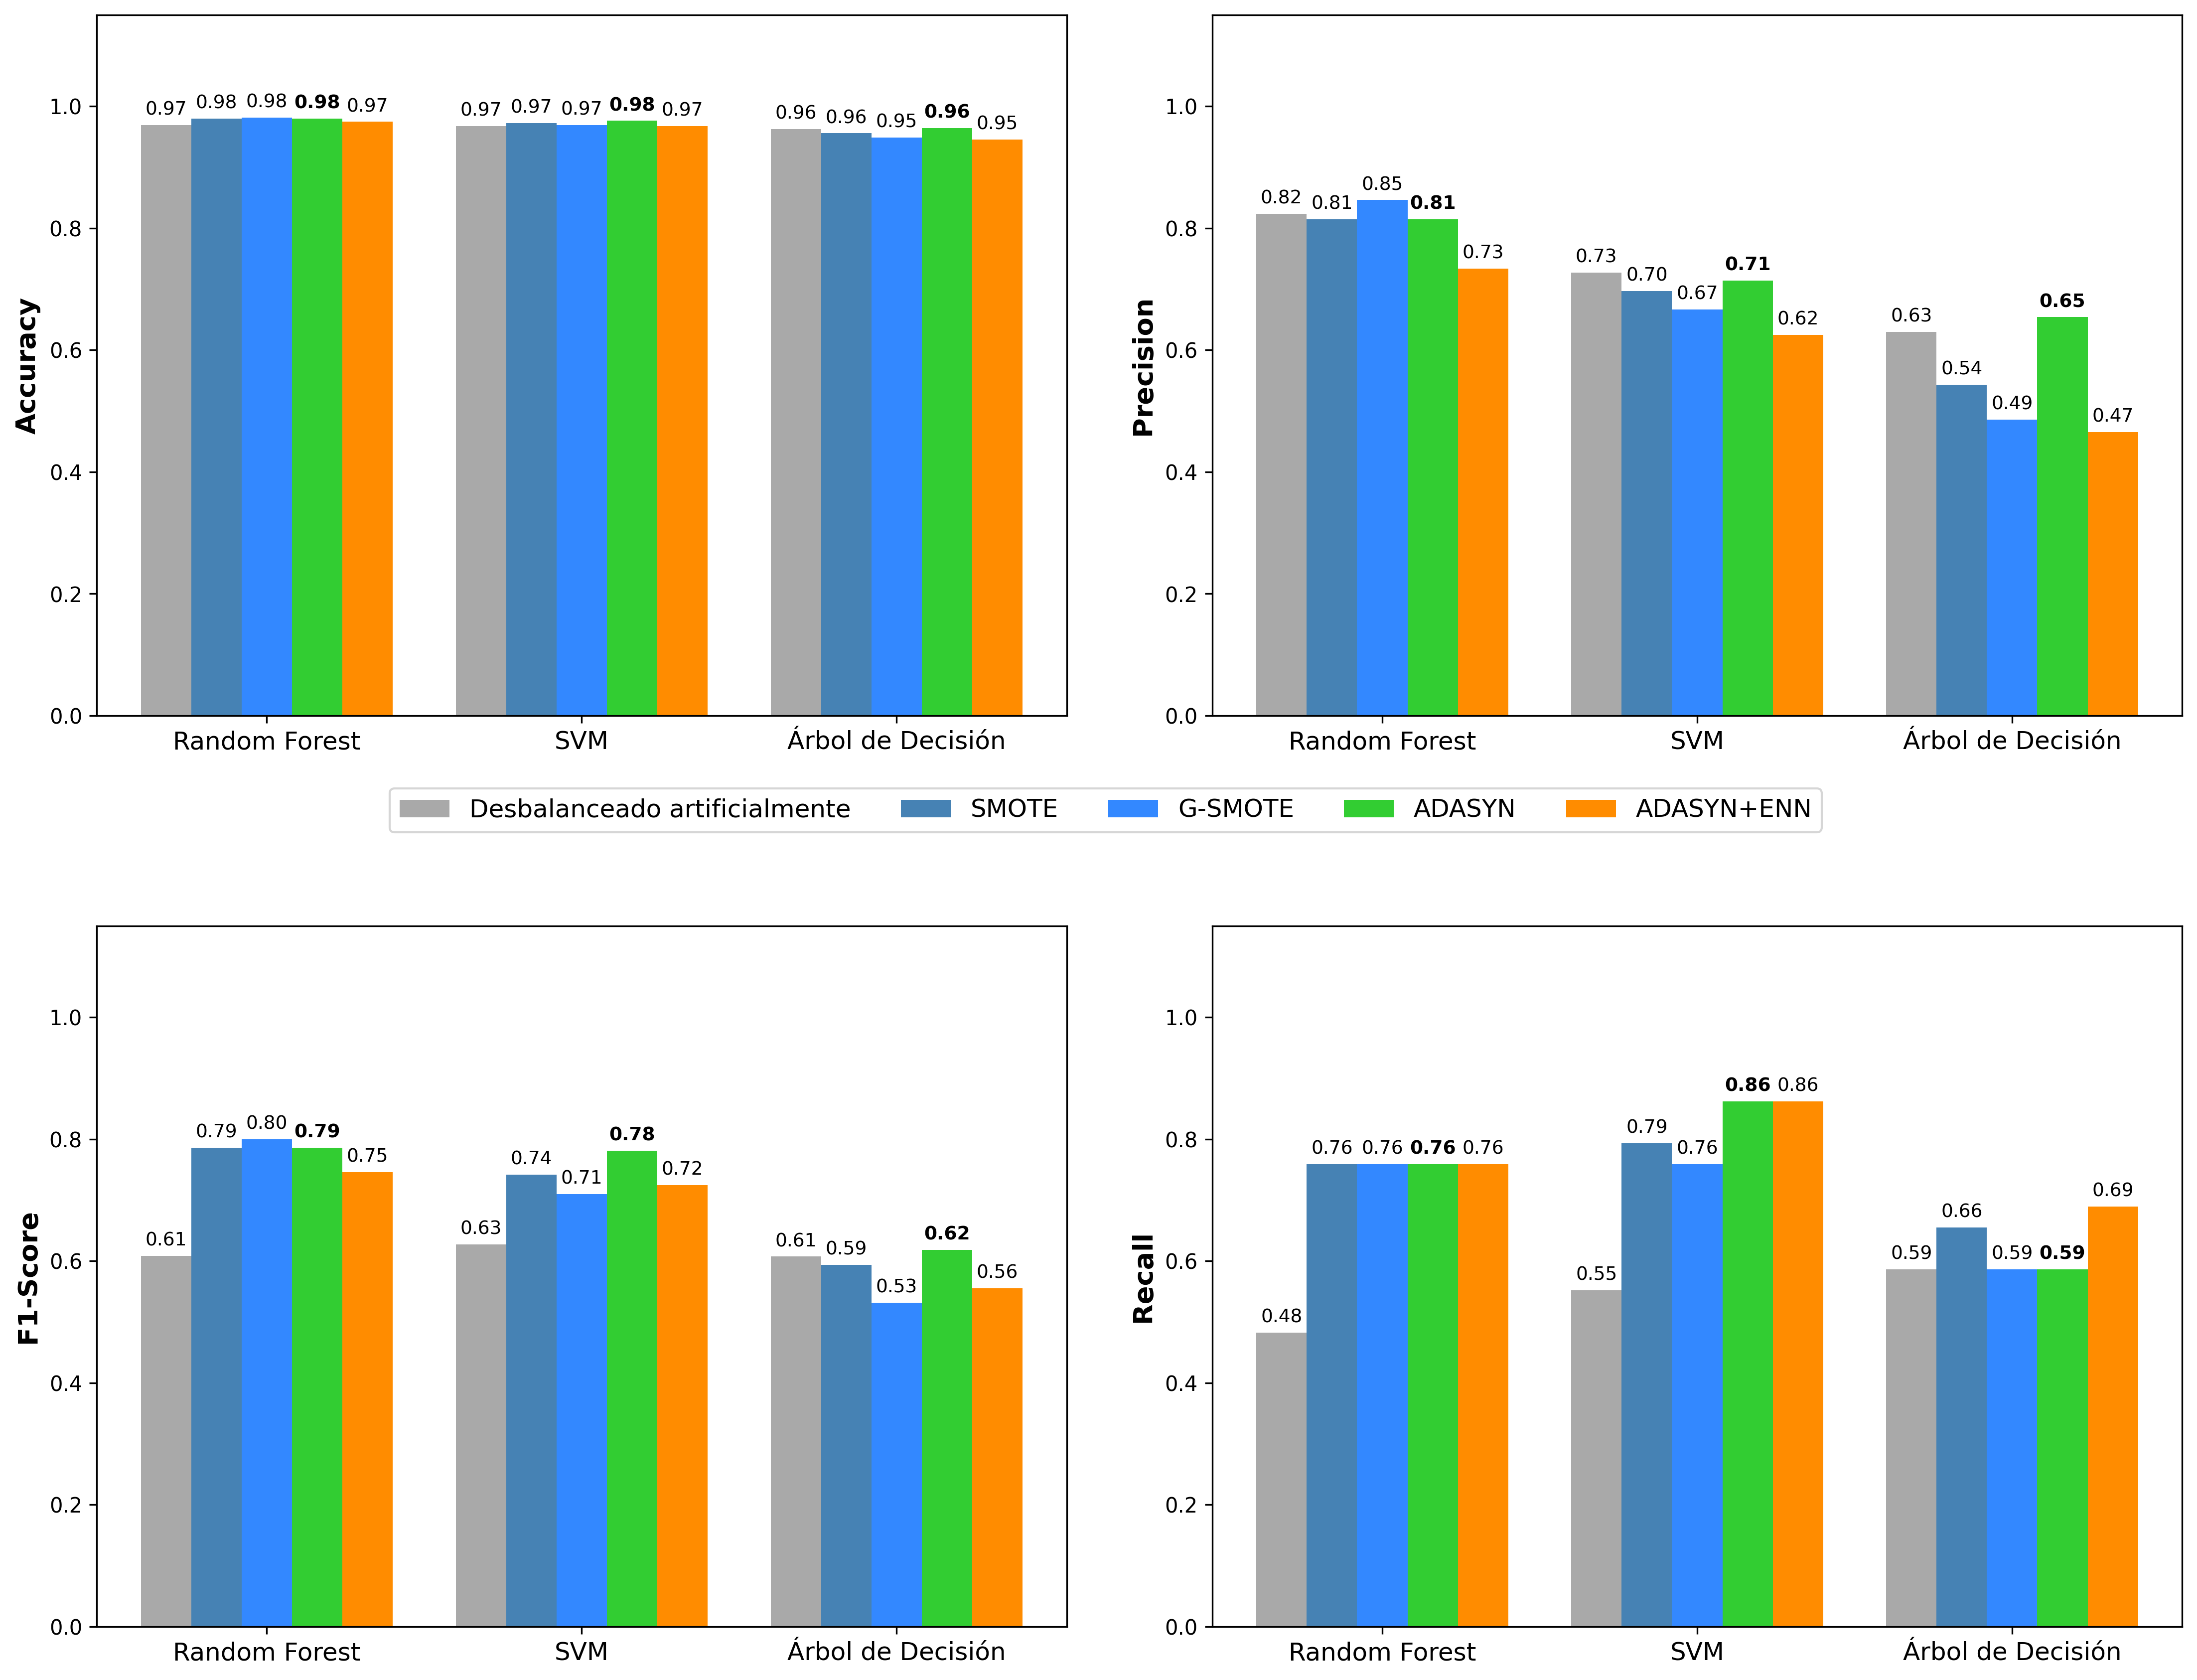
\includegraphics[width=\textwidth,height=0.75\textheight,keepaspectratio]{metricas_7030_unificadas.png}
  \end{figure}
  \vspace{-0.5cm}
  \begin{itemize}\scriptsize
    \item \textbf{Random Forest (G-SMOTE):} Alcanzó la mayor Precision (\textbf{0,84}) y el mejor F1-Score (\textbf{0,80}).
    \item \textbf{SVM (ADASYN):} Logró el mayor Recall, con un valor de \textbf{0,86}.
  \end{itemize}
\end{frame}

\begin{frame}{Comparativa: Sobremuestreo vs. Datos Originales}
  \begin{figure}
    \centering
    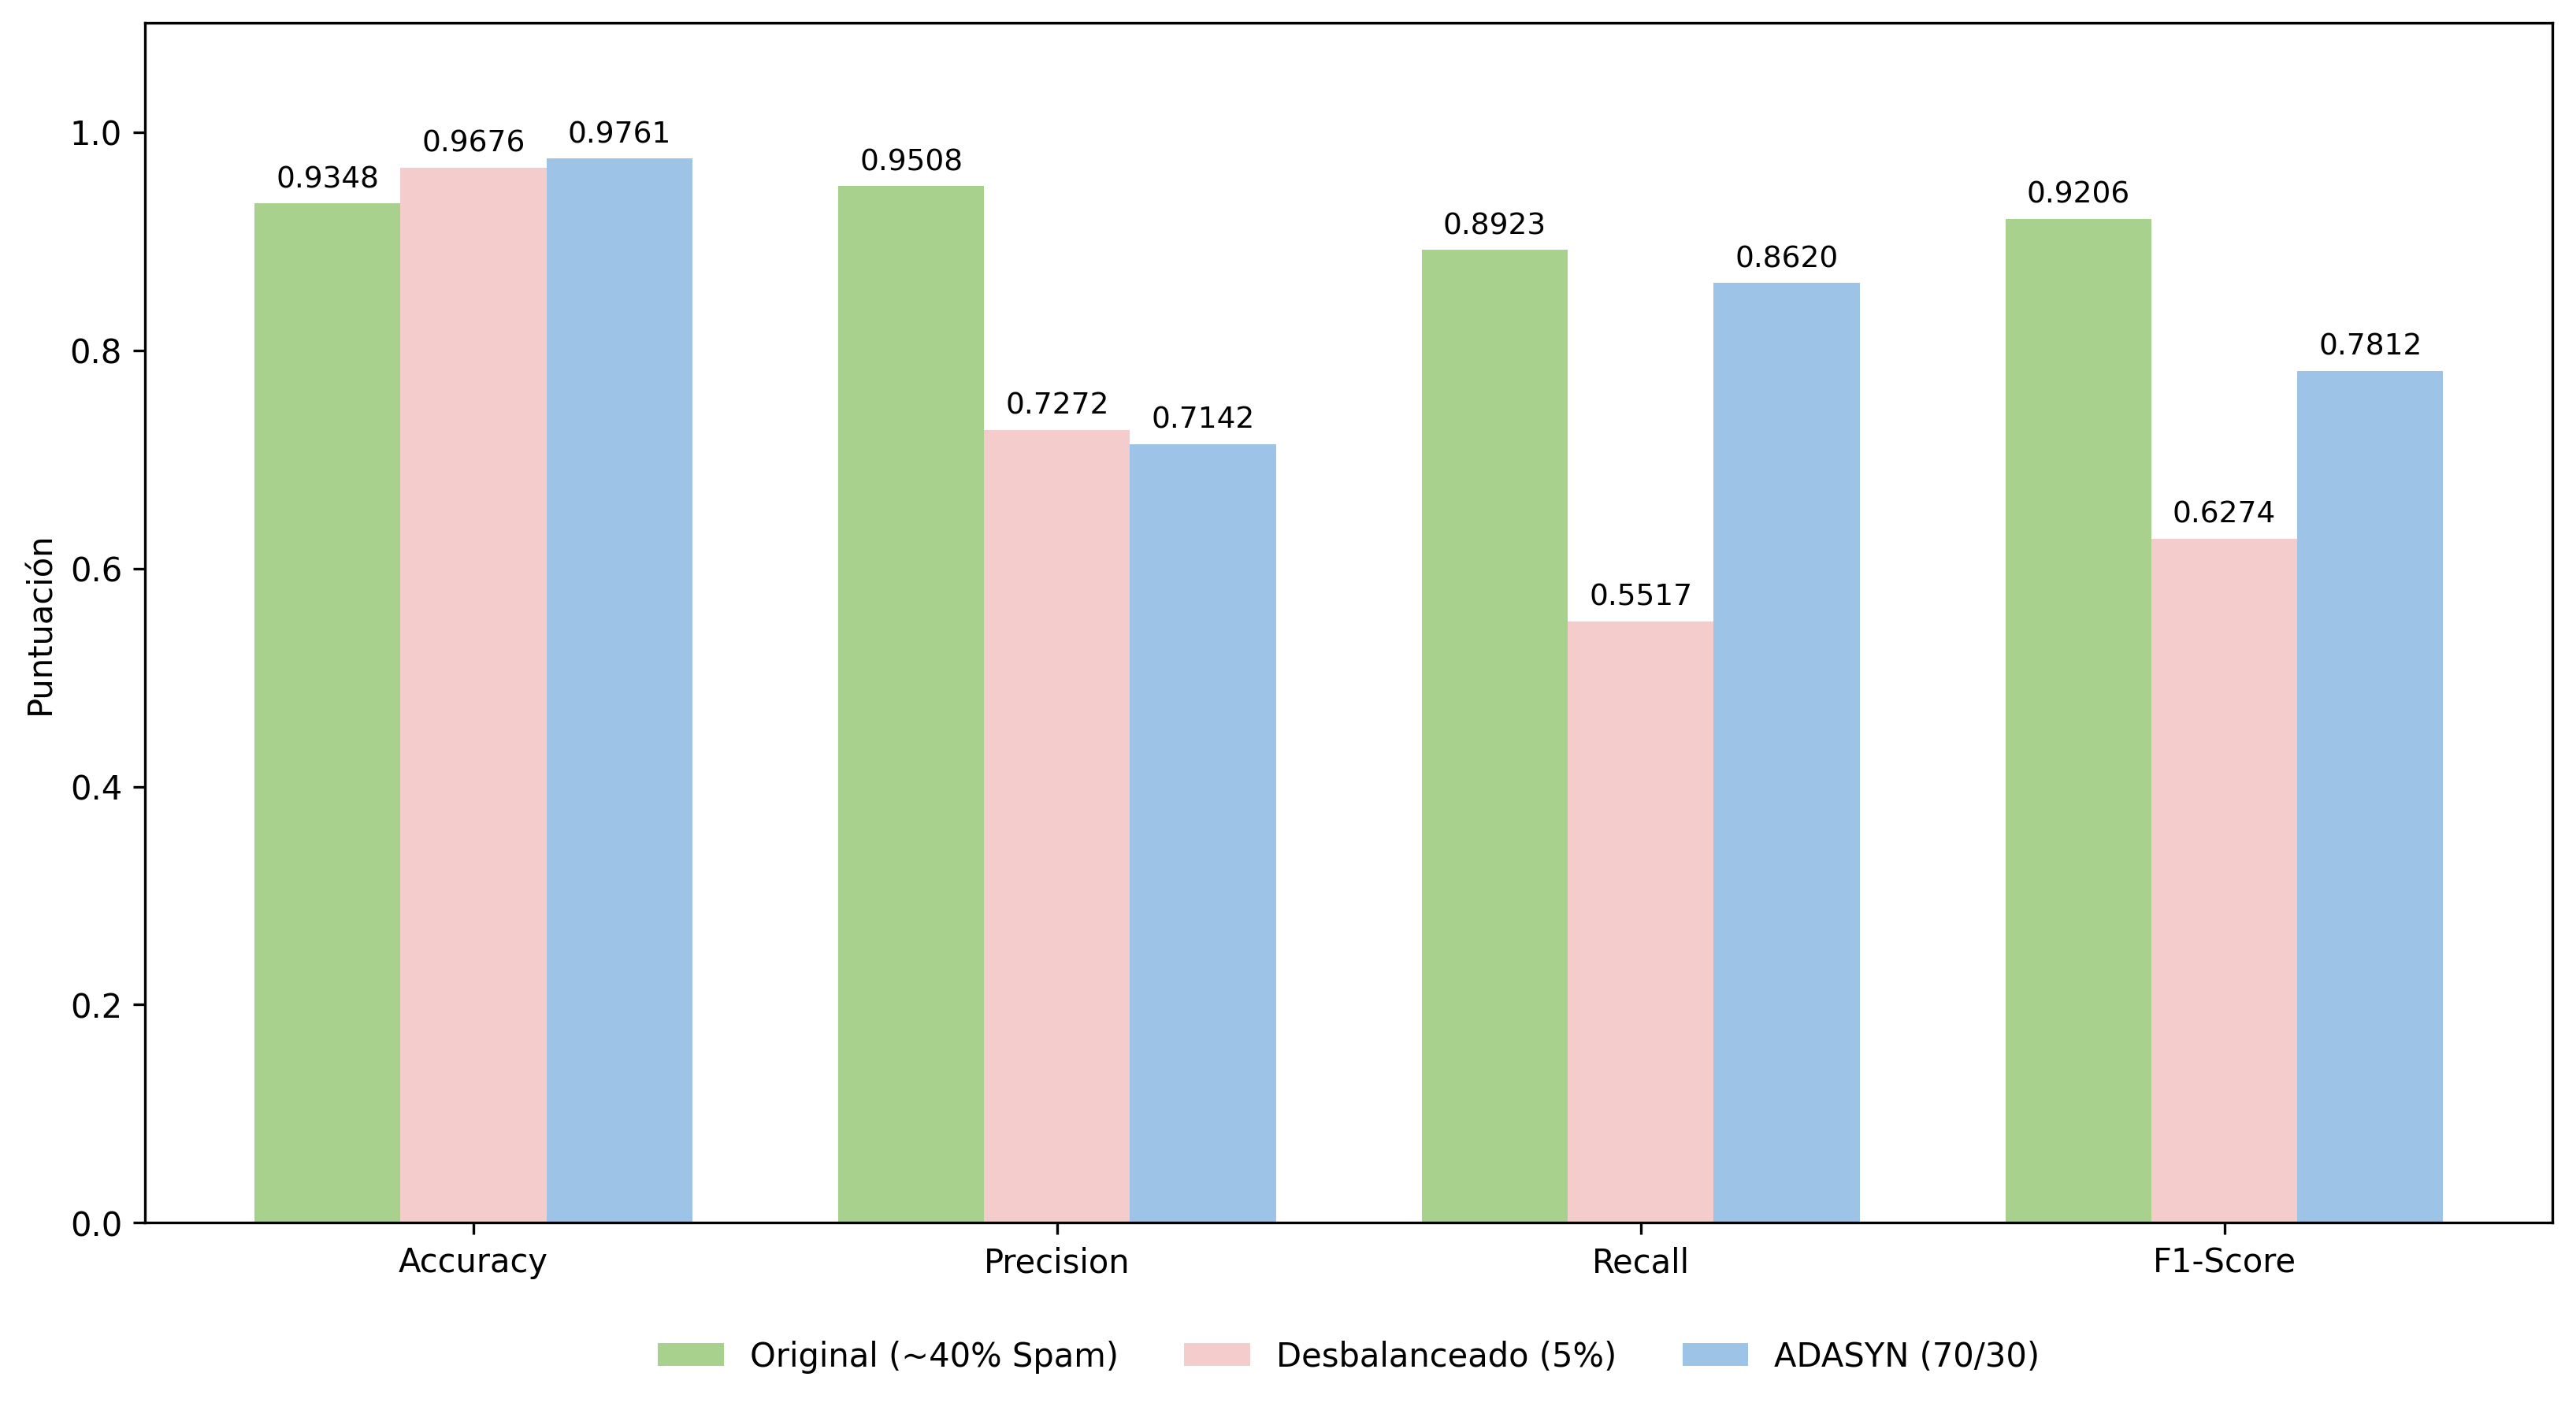
\includegraphics[width=\textwidth,height=0.7\textheight,keepaspectratio]{comparativa_original_vs_7030.png}
  \end{figure}
  \vspace{-0.5cm}
  \textbf{\scriptsize Impacto del Sobremuestreo (SVM + ADASYN):}
  \begin{itemize}\scriptsize
    \item Al aplicar ADASYN (70-30), el modelo eleva su Recall a 0,86.
    \item Se aproxima fuertemente al rendimiento del modelo entrenado con el dataset original (Recall de 0,89), superando ampliamente al desbalanceado.
  \end{itemize}
\end{frame}

\section{Conclusiones}

\begin{frame}{Conclusiones: Los Mejores resultados}
  No existe un sobremuestreo perfecto; el ganador depende de la prioridad buscada.
  \vspace{0.4cm}
  
  \textbf{1. Prioridad: Minimizar Falsos Positivos} 
  \begin{itemize}
      \item \textbf{Ganador:} Random Forest + G-SMOTE
      \item Gracias a la restricción esférica, alcanzó la mejor Precision (0,84) y el mejor F1-Score (0,80) del estudio.
  \end{itemize}

  \vspace{0.3cm}
  \textbf{2. Prioridad: Máxima Detección} 
  \begin{itemize}
      \item \textbf{Ganador:} SVM (Umbral ajustado a 0.2) + ADASYN
      \item Enfoque si se prioriza detectar amenazas. Logró un  Recall de 0,86, detectando casi todas las amenazas a costo de permitir más falsos positivos.
  \end{itemize}
\end{frame}

\begin{frame}{Conclusiones: Sobremuestreo vs. Datos Reales}
  \begin{itemize}
    \item \textbf{Comparativa Final:} 
    Se evaluó el método de sobremuestreo ganador contra el conjunto \textit{SpamBase original} el cual poseía naturalmente un 40\% de spam.
    \vspace{0.2cm}
    \item \textbf{Original vs Sobremuestreado:} 
    Lógicamente, los datos originales demostraron una ligera superioridad (Recall de 0,89). 
    \vspace{0.2cm}
    \item Sin embargo, el modelo entrenado con ADASYN logró un Recall de 0,86 partiendo desde un desbalance del 5\%. 
    \vspace{0.2cm}
    \item \textbf{Reflexión Final:} Esto demuestra que las técnicas de sobremuestreo son herramientas eficaces y robustas, capaces de recuperar casi por completo la capacidad predictiva de algoritmos limitados por la carencia de observaciones.
  \end{itemize}
\end{frame}

\begin{frame}[standout]
  ¡Muchas gracias!
\end{frame}

\end{document}
